% Enable warnings about problematic code
\RequirePackage[l2tabu, orthodox]{nag}

\documentclass{WeSTassignment}

\usepackage{listings}
\usepackage{color}

\definecolor{dkgreen}{rgb}{0,0.6,0}
\definecolor{gray}{rgb}{0.5,0.5,0.5}
\definecolor{mauve}{rgb}{0.58,0,0.82}

\lstset{frame=tb,
  language=python,
  aboveskip=3mm,
  belowskip=3mm,
  showstringspaces=false,
  columns=flexible,
  basicstyle={\small\ttfamily},
  numbers=none,
  numberstyle=\tiny\color{gray},
  keywordstyle=\color{blue},
  commentstyle=\color{dkgreen},
  stringstyle=\color{mauve},
  breaklines=true,
  breakatwhitespace=true,
  tabsize=2
}


% The lecture title, e.g. "Web Information Retrieval".
\lecture{Introduction to Web Science}
% The names of the lecturer and the instructor(s)
\author{%
  Prof. Dr.~Steffen~Staab\\{\normalsize\mailto{staab@uni-koblenz.de}} \and
  Ren{\'e}~Pickhardt\\{\normalsize\mailto{rpickhardt@uni-koblenz.de}} \and
   Korok~Sengupta\\{\normalsize\mailto{koroksengupta@uni-koblenz.de}} \and 
   Olga~Zagovora\\{\normalsize\mailto{zagovora@uni-koblenz.de}}
}
% Assignment number.
\assignmentnumber{8}
% Institute of lecture.
\institute{%
  Institute of Web Science and Technologies\\%
  Department of Computer Science\\%
  University of Koblenz-Landau%
}
% Date until students should submit their solutions.
\datesubmission{January 11, 2017, 10:00 a.m.}
% Date on which the assignments will be discussed in the tutorial.
\datetutorial{January 13, 2017, 12:00 p.m.}

% Set langauge of text.
\setdefaultlanguage[
  variant = american, % Use American instead of Britsh English.
]{english}

% Specify bib file location.
\addbibresource{bibliography.bib}

% For left aligned centerd boxes
% see http://tex.stackexchange.com/a/25591/75225
\usepackage{varwidth}
% ==============================================================================
% Document

\begin{document}

\maketitle
Please look at all the lessons of part 2 in particular \textbf{Similarity of Text} and \textbf{graph based models}

For all the assignment questions that require you to write code, make sure to include the code in the answer sheet, along with a separate python file. Where screen shots are required, please add them in the answers directly and not as separate files.\\ \\ 

Other than that this sheet is mainly designed to review and apply what you have learnt in part 2 it is a little bit larger but there is also more time over the x-mas break. In any case we wish you a mery x-mas and a happy new year. 

%Please mention your team Names here: 
Team Name: papa \\
Members: Brigitte Aznar \\
Bonasmitha Behura \\
Ilia Tugushi


\section{Similarity - (40 Points)}
This assignment will have one exercise which is dived into four subparts. 
The main idea is to study once again the web crawl of the Simple English Wikipedia. The goal is also to review and aply your knowledge from part 2 of this course.

We have constructed two data sets from it which are all the articles and the link graph extracted from Simple English Wikipedia. The extracted data sets are stored in the file \url{http://141.26.208.82/store.zip} which contains a pandas container and can be read with pandas in python. In subsection ``1.5 Hints"  you will find some sample python code that demonstrates how to easily access the data.

With this data set you will create three different models with different similarity measures and finally try to evaluate how similar these models are. 

\textbf{This assignment requires you to handle your data in efficient data structures otherwise you might discover runtime issues. So please read and understand the full assignment sheet with all the tasks that are required before you start implementing some of the tasks.}

\subsection{Similarity of Text documents  (10 Points)}
\subsubsection{Jaccard - Similarity on sets}
\begin{enumerate}
\item Build the word sets of each article for each article id.
\item Implement a function \texttt{calcJaccardSimilarity(wordset1, wordset2)} that can calculate the jaccard coefficent of two word sets and return the value.
\item Compute the result for the articles \texttt{Germany} and \texttt{Europe}.\\
\end{enumerate}
\textbf{Answer:}\\
The Jaccard similarity for Germany and Europe is 0.0444

\subsubsection{TF-IDF with cosine similarity}
\begin{enumerate}
\item Count the term frequency of each term for each article
\item Count the document frequencies of each term. 
\item For each article id provide a dictionary of terms occuring in the article together with their tf-idf scores as the corresponding values.
\item Implement a function \texttt{calculateCosineSimilarity(tfIdfDict1, tfIdfDict2)} that computes the cosine similarity for two sparse tf-idf vectors and returns the value.
\item Compute the result for the articles \texttt{Germany} and \texttt{Europe}.\\
\end{enumerate}
\textbf{Answer:}\\
The Cosine similarity for Germany and Europe is 0.1803
\subsection{Similarity of Graphs (10 Points)}
You can understand the similarity of two articles by comparing their sets of outlinks (and see how much they have in common). Feel free to reuse the \texttt{computeJaccardSimilarity} function from the first part of the exercise. This time do not aply it on the set of words within two articles but rather on the set of outlinks being used within two articles. Again compute the result for the articles \texttt{Germany} and \texttt{Europe}.\\
\textbf{Answer:}\\
The Jaccard similarity for Germany and Europe (Out links) is 0.2731

\subsection{How similar have our similarities been? (10 Points)}
Having implemented these three models and similarity measures (text with Jaccard, text with cosine, graph with Jaccard) our goal is to understand and quantify what is going on if they are used in the wild. Therefore in this and the next subtask we want to try to give an answere to the following questions.

\begin{itemize}
\item Will the most similar articles to a certain article always be the same independent which model we use? \\\\
\textbf{Answer:}\\
No. As running the code we can see in the file 'compare100.txt', and in the function 'compareAll' that the most similar article from 100 random articles to one pre selected article in this case Germany, is not the same when is it run with two different similarity measures (Jaccard and Cosine) 

How ever yet if not the same we can see that the two different models have a similar pattern.

\begin{figure}[h!]
  \centering
  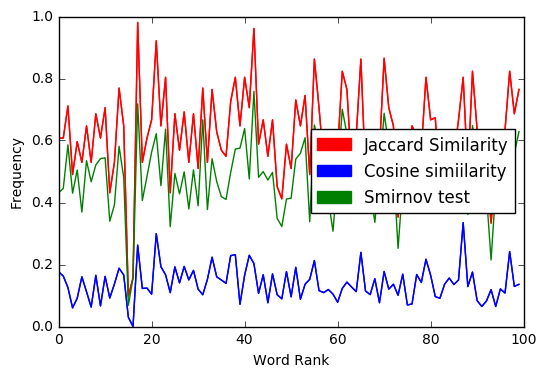
\includegraphics[scale=0.5]{compare.png}
   \caption{visiualization of similarities}
     \label{fig:dig} 
\end{figure}
\item How similar are these measures to each other? How can you statistically compare them?\\ \\ \\\\
\textbf{Answer:}\\\\
We ran a Kolmogorov–Smirnov test to compare the similarities.
We used this method because it calculates the distance between two values so it tells us in a simple way how far apart are from each other.
\end{itemize}

Assume you could use the similarity measure to compute the top k most similar articles for each article in the document collection. We want to analyze how different the rankings for these various models are. 

Do some research to find a statistical measure (either from the lectures of part 2 or by doing a web search and coming up with something that we haven't discussed yet) that could be used best to compare various rankings for the same object. 

Explain in a short text which measure you would use in such an experiment and why you think it is usefull for our task. 

\subsection{Implement the measure and do the experiment (10 Points)}
After you came up with a measure you will most likely run into another problem when you plan to do the experiment. 

Since runtime is an issue we cannot compute the similarity for all pairs of articles. Tell us: 
\begin{enumerate}
\item How many similarity computations would have to be done if you wished to do so? 
\begin{enumerate}
\item We estimate that 756085009 computations are needed to compare the whole data set
\end{enumerate}
\item How much time would roughly be consumed to do all of these computations?
\begin{enumerate}
\item to calculate the similarities from 100 articles to a single article took 9.18 minutes which means that to calculate all the similarities it would be needed around 4162907860.86 minutes
\end{enumerate}
\end{enumerate}

A better strategy might be to select a couple of articles for which you could compute your meassure. One strategy would be to select the 100 longest articles. Another strategy might be to randomly select 100 articles from our corpus. 

Computer your three similarity measures and evaluate them for these two strategies of selecting test data. Present your results. Will the results depend on the method for selecting articles? What are your findings? \\\\
\textbf{Answer:}\\
As we can see in the graphs when we use the largest 100 articles, they are more similar to 'Germany' than if we just take random 100 articles.
This is because in larger articles there are of course more words and therefor there is a highest chance that this words are present in our base document in this case 'Germany'. \\\\
\begin{figure}[h]
  \centering
  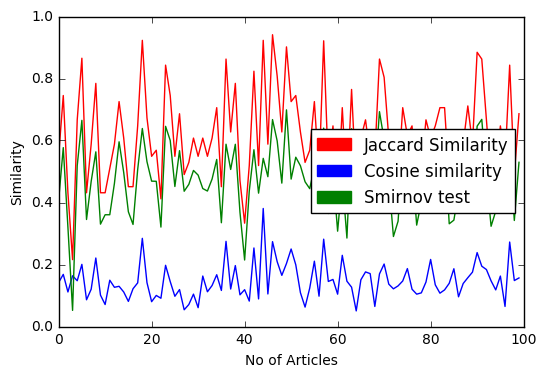
\includegraphics[scale=0.5]{comparerandom.png}
   \caption{visiualization of similarities for 100 random articles vs Germany}
     \label{fig:dig} 
\end{figure}

\begin{figure}[h]
  \centering
  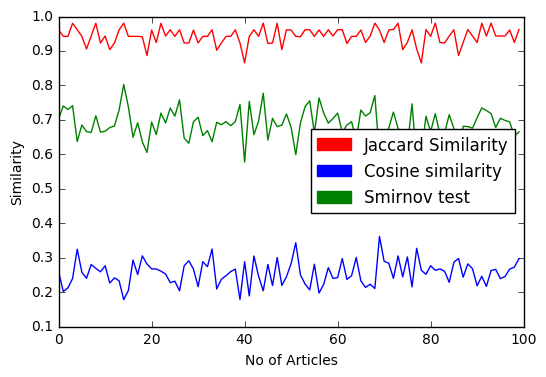
\includegraphics[scale=0.5]{comparetop100.png}
   \caption{visiualization of similarities for top 100 largest articles vs Germany}
     \label{fig:dig} 
\end{figure}


\begin{lstlisting}

# coding: utf-8

# In[19]:

from __future__ import division
import os
import re
import yaml
import math
import time
import random
import numpy as np
import pandas as pd
from collections import Counter
import matplotlib.pyplot as plt
import matplotlib.patches as mpatches


# In[20]:

store = pd.HDFStore('store.h5')
df1 = store['df1']
df2 = store['df2']


# In[21]:

path_to_file = os.path.realpath('.')


# In[22]:

def getSets(df, index1, index2):
    total_words = 0
    i = 0 
    set1 = set()
    set2 = set()
    if 'text' in df.columns:
        for words in df.text[index1]:
            re_words = re.findall(r'\b[^\d\W]+\b', words)
            for word in re_words:
                set1.add(word)
        for words in df.text[index2]:
            re_words = re.findall(r'\b[^\d\W]+\b', words)
            for word in re_words:
                set2.add(word)
    else:
        for words in df.out_links[index1]:
            for word in words:
                set1.add(word)
        for words in df.out_links[index2]:
            for word in words:
                set2.add(word)
    return set1, set2


# In[23]:

def countTFPerArticle(df):
    i = 0
    text_to_write = ''
    for article in df.text:
        j = 0
        re_words = re.findall(r'\b[^\d\W]+\b', article)
        re_words =  [x.lower() for x in re_words]
        counter = Counter(re_words)
        try:
            words, frqs = zip(*counter.most_common())
            text_to_write += df.name[i] + '= {' 
            while j < len(words):
                text_to_write +=  "'" + words[j] + "'" + ': ' + str(frqs[j]) +', '
                j += 1
                
        except Exception as e:
            pass        
        text_to_write += '}\r\n'
        i += 1
        
        if i%1000 == 0:
            with open(os.path.join(path_to_file, 'tf_per_article_dict.txt'), 'a') as file_to_write:
                file_to_write.write(text_to_write)
                file_to_write.close()
            text_to_write = ''
    with open(os.path.join(path_to_file, 'tf_per_article_dict.txt'), 'a') as file_to_write:
        file_to_write.write(text_to_write)
        file_to_write.close()


# In[24]:

def countTFPerDoc(df):
    j = 0
    text_to_write = ''
    allwords = []
    for article in df.text:
        allwords += re.findall(r'\b[^\d\W]+\b', article)
    allwords =  [x.lower() for x in allwords]

    try:
        counter = Counter(allwords)
        words, frqs = zip(*counter.most_common())
    except Exception:
        pass
    text_to_write = '{'
    while j < len(words):
        text_to_write +=  "'" + words[j] + "'" + ': ' + str(frqs[j]) +', '
        j += 1
        if j%1000 == 0:
            with open(os.path.join(path_to_file, 'tf_per_doc.txt'), 'a') as file_to_write:
                file_to_write.write(text_to_write)
                file_to_write.close()
            text_to_write = ''
    text_to_write = '}'
    with open(os.path.join(path_to_file, 'tf_per_doc.txt'), 'a') as file_to_write:
        file_to_write.write(text_to_write)
        file_to_write.close()


# In[25]:

def calcJaccardSimilarity(set1, set2):
    inter = 0
    union_set = set1.union(set2)
    union = len(union_set)
    for word in set1:
        if word in set2:
            inter += 1    

    return round(inter/union,4)


# In[26]:

def calcTFIDF(df, dict1, dict2, dictN):
    corpus_len = len(df)
    dict_tfidf1 = {}
    dict_tfidf2 = {}

    #number of docs where the term x appears

    for key in dictN:
        #Doc1
        for key1 in dict1:
            if key1 == key:
                dict_tfidf1.update({key:dict1[key]/len(dict1) * math.log10(corpus_len/dictN[key]) })
        #Doc2
        for key2 in dict2:
            if key2 == key:
                dict_tfidf2.update({key: dict2[key]/len(dict2) * math.log10(corpus_len/dictN[key]) })
        
    return dict_tfidf1, dict_tfidf2


# In[27]:

def calculateCosineSimilarity(tfidf1, tfidf2):
    v1 = []
    v2 = []
    vset1 = []
    vset2 = []
    dotp = 0
    i = 0
    for key1 in tfidf1:
        vset1.append(key1)
    for key2 in tfidf2:
        vset2.append(key2)
    #Get the sparse vectors
    for key1 in tfidf1:
        v1.append(1)
        if key1 in vset2:
            v2.append(1)
            del tfidf2[key1]
        else:
            v2.append(0)
    
    for key2 in tfidf2:
        v2.append(1)
        if key2 in vset1:
            v1.append(1)
        else:
            v1.append(0)
    
    #Get dot product
    while i < len(v1):
        dotp += v1[i]*v2[i]
        i += 1
    #Get the norms
    norm1 = math.sqrt(sum(v1))
    norm2 = math.sqrt(sum(v2))
    #calculate cos similarity
    cos_sim = dotp/(norm1*norm2)
    
    return round(cos_sim,4)


# In[28]:

def dictionarize(name1, name2):
    dictN = {}
    name1 += '='
    name2 += '='
    dict1 = dict()
    dict2 = dict()
    size = 0
    file = open(os.path.join(path_to_file, 'tf_per_article_dict.txt'), 'r')
    for line in file:
        size += 1
        if name1 in line:
            name, words = line.split("=",1)
            words = words.replace(', }', '}')
            dict1 =yaml.load(words)
        if name2 in line:
            name, words = line.split("=",1)
            words = words.replace(', }', '}')
            dict2 =yaml.load(words)
        re_words = re.findall(r'\b[^\d\W]+\b', line)
        for re_word in re_words:
            if re_word in dictN:
                #Counts number of docs the word X appears
                dictN[re_word] += 1
            else:
                dictN.update({re_word: 1}) 
    file = open(os.path.join(path_to_file, 'tf_per_doc.txt'), 'r')
    for line in file:  
        words = words.replace(', }', '}')
        dict_all =yaml.load(words)
    return dict1, dict2, dict_all, dictN, size


# In[29]:

def getIndexes(index1):
    index2 = random.randint(0,len(df1))
    while df1.text[index2] == '':
        index2 = random.randint(0,len(df1))
    if index1 == index2:
        if index1 == len(df1) -1:
            index2 = index2 -1
        else:
            index2 += 1
    return index2


# In[30]:

def getLongest():
    length = []
    indexes = []
    for article in df1.text:
        length.append(len(article))
    for index in df1.index:
        indexes.append(index)
    
    list1, list2 = zip(*sorted(zip(length, indexes), reverse=True))
    return list(list2[:100])


# In[31]:

def compareAll():
    cos = []
    jacc = []
    file = open(os.path.join(path_to_file, 'compare.txt'), 'r')
    for line in file:
        jacca = line.find('jaccard')
        jacc.append(line[jacca + len('jaccard') + 2 : line.find(',', jacca)] )
        cosi = line.find('cosine')
        cos.append(line[cosi + len('cosine') + 2 :line.find('}', cosi)])

    if np.argmax(jacc) == np.argmax(cos):
        print 'The most similar articles to a certain article always be the same independent which model we use'
    else:
        print 'With different models we get different articles'
    try:
        smirnov = [float(jacc1) - float(cos1) for jacc1, cos1 in zip(jacc, cos)]
    except Exception:
        pass        
    return smirnov


# In[32]:

def buildRandom():
    i = 0
    text_to_write = ''
    index1 = 27444 #germany
    jaccardl = []
    cosinel = []
    while i < 100:
        index2 = getIndexes(index1)
        set1, set2 = getSets(df1, index1, index2)
        jaccard = calcJaccardSimilarity(set1, set2)
        dict11, dict21, dictall1, dictN1, size = dictionarize(df1.name[index1], df1.name[index2])
        tdfidf11, tdfidf21 = calcTFIDF(df1,dict11,dict21,dictN1)
        cos_sim = calculateCosineSimilarity(tdfidf11, tdfidf21)
        jaccardl.append(jaccard)
        cosinel.append(cos_sim)
        text_to_write += "{" + df1.name[index1]+ ":{" +df1.name[index2] + ":{" + "\'jaccard\':" + str(jaccard) + ", \'cosine\':" + str(cos_sim)+ '}}} \r\n'
        i += 1
    with open(os.path.join(path_to_file, 'compare.txt'), 'w') as file_to_write:
        file_to_write.write(text_to_write)
        file_to_write.close()
    return jaccardl, cosinel


# In[33]:

def buildLongest():
    i = 0
    text_to_write = ''
    index1 = 27444 #germany
    jaccardl = []
    cosinel = []
    longest = getLongest()
    while i < 100:
        index2 = longest.pop()
        set1, set2 = getSets(df1, index1, index2)
        jaccard = calcJaccardSimilarity(set1, set2)
        dict11, dict21, dictall1, dictN1, size = dictionarize(df1.name[index1], df1.name[index2])
        tdfidf11, tdfidf21 = calcTFIDF(df1,dict11,dict21,dictN1)
        cos_sim = calculateCosineSimilarity(tdfidf11, tdfidf21)
        jaccardl.append(jaccard)
        cosinel.append(cos_sim)
        text_to_write += "{" + df1.name[index1]+ ":{" +df1.name[index2] + ":{" + "\'jaccard\':" + str(jaccard) + ", \'cosine\':" + str(cos_sim)+ '}}} \r\n'
        i += 1
    with open(os.path.join(path_to_file, 'compare.txt'), 'w') as file_to_write:
        file_to_write.write(text_to_write)
        file_to_write.close()
    return jaccardl, cosinel


# In[34]:

index1 = df1.index[df1.name=="Germany"]
index2 = df1.index[df1.name=="Europe"]
set1, set2 = getSets(df1, index1, index2)


# In[17]:

jaccard = calcJaccardSimilarity(set1, set2)
print 'Jaccard similarity for Germany and Europe is ' + str(jaccard)


# In[18]:

if not os.path.isfile('tf_per_article_dict.txt'):
    countTFPerArticle(df1)


# In[136]:

if not os.path.isfile('tf_per_doc.txt'):
    countTFPerDoc(df1)


# In[35]:

dict1, dict2, dictall, dictN, size = dictionarize('Germany', 'Europe')


# In[36]:

tdfidf1, tdfidf2 = calcTFIDF(df1,dict1,dict2,dictN)


# In[37]:

cos_sim = calculateCosineSimilarity(tdfidf1, tdfidf2)
print 'Cosine similarity for Germany and Europe is ' + str(cos_sim)


# In[38]:

set1, set2 = getSets(df2, index1, index2)
jaccard = calcJaccardSimilarity(set1, set2)
print 'Jaccard similarity for Germany and Europe (Out links) is ' + str(jaccard)


# In[39]:

before = time.clock()
jaccardl, cosinel = buildRandom()
after = time.clock()


# In[40]:

comparisson = compareAll()


# In[41]:

elapsed_time = after - before
print 'Elapsed time to calculate 100 similarities ' + str(round(elapsed_time/60,2)) + ' minutes'


# In[42]:

time_for_all_to_one = size * elapsed_time / 100
time_for_all = time_for_all_to_one * size
print str(time_for_all) + ' minutes'


# In[43]:

plt.plot(jaccardl, 'r-')
plt.plot(cosinel, 'b-')
plt.plot(comparisson, 'g-')

# adds labels to the axis
plt.ylabel('Similarity')
plt.xlabel('No of Articles')
# generates legend
jacc_legend = mpatches.Patch(color='red', label='Jaccard Similarity')
cos_legend = mpatches.Patch(color='blue', label='Cosine similarity')
comp_legend = mpatches.Patch(color='green', label='Smirnov test')
plt.legend(handles=[jacc_legend, cos_legend, comp_legend ], loc=5)
plt.show()


# In[44]:

before = time.clock()
jaccardl, cosinel = buildLongest()
after = time.clock()


# In[45]:

comparisson = compareAll()


# In[46]:

total_computations = size * size
print total_computations


# In[47]:

plt.plot(jaccardl, 'r-')
plt.plot(cosinel, 'b-')
plt.plot(comparisson, 'g-')

# adds labels to the axis
plt.ylabel('Similarity')
plt.xlabel('No of Articles')
# generates legend
jacc_legend = mpatches.Patch(color='red', label='Jaccard Similarity')
cos_legend = mpatches.Patch(color='blue', label='Cosine similarity')
comp_legend = mpatches.Patch(color='green', label='Smirnov test')
plt.legend(handles=[jacc_legend, cos_legend, comp_legend ], loc=5)
plt.show()


\end{lstlisting}
\subsection{Hints:}
\begin{enumerate}
\item In oder to access the data in python, you can use the following pice of code:
\begin{lstlisting}
import pandas as pd
store = pd.HDFStore('store.h5')
df1=store['df1'] 
df2=store['df2'] 
\end{lstlisting}
\item Variables df1 and df2 are pandas DataFrames which is tabular data structure. df1 consists of article's texts, df2 represents links from Simple English Wikipedia articles. Variables have the following columns:
\begin{itemize}
\item ``name" is a name of Simple English Wikipedia article,
\item ``text" is a full text of the article ``name",
\item ``out\_links" is a list of article names where the article ``name" links to.
\end{itemize}
\item In general you might want to store the counted results in a file before you do the similarity computations and all the research for the third and fourth subtask. Doing all this counting and preperation might allready take quite some runtime. 
\item When computing the sparse tf-idf vectors you might allready want to store the eukleadan length of the vectors. otherwise you might discover runtime issues when computing the length again for each similarity computation. 
\item Finding the top similar articles for a given article id requires you to compute the similarity of the given article with comparison to all the other known articles and extract the top 5 similarities. Bare in mind that these are quite a lot of similarity computations! You can expect a runtime to find the top similar articles with respect to one of the methods to be up to 10 seconds. If it takes significant longer then you probably have not used the best data structures handle your data.
\item \textbf{Even though many third party libraries exist to do this task with even less computational effort those libraries must not be used.}
\item You can find more information about basic usage of pandas DataFrame in  \href{http://pandas.pydata.org/pandas-docs/stable/dsintro.html#column-selection-addition-deletion}{pandas documentation}.
\item Here are some usefull examples of operations with DataFrame:
\begin{lstlisting} 
import pandas as pd

store = pd.HDFStore('store.h5')#read .h5 file
df1=store['df1'] 
df2=store['df2'] 
print df1['name'] # select column "name"
print df1.name # select column "name"
print df1.loc[9] #select row with id equals 9 
print df1[5:10] #select rows from 6th to 9th (first row is 0) 
print df2.loc[0].out_links #select outlinks of article with id=0 

#show all columns where column "name" equals "Germany"
print df2[df2.name=="Germany"]

#show column out_links for rows where name is from list ["Germany","Austria"]
print df2[df2.name.isin(["Germany","Austria"])].out_links 

#show all columns where column "text" contains word "good" 
print df1[df1.text.str.contains("good")]

#add word "city" to the beginning of each text value 
#(IT IS ONLY SHOWS RESULT OF OPERATION, see explanation below!)
print df1.text.apply(lambda x: "city "+x)

#make all text lower case and split text by spaces
df1[["text"]]=df1.text.str.lower().str.split()

def do_sth(x):
	#here is your function
	#
	#
	return x
    
#apply do_sth function to text column 
#Iit will not change column itself, it will only show the result of aplication	
print df1.text.apply(do_sth())

#you always have to assign result to , e.g., column, 
#in order it affects your data.
#Some functions indeed can change the DataFrame by 
#applying them with argument inplace=True
df1[["text"]]=df1.text.apply(do_sth())  

#delete column "text"
df1.drop('text', axis=1, inplace=True)
\end{lstlisting}

\end{enumerate}







\makefooter

\end{document}
